\documentclass[14pt, aspectratio=169]{beamer}
\usetheme{Copenhagen}

\usepackage{graphicx}
\usepackage{forest}
\usepackage{tikz}
\usetikzlibrary{positioning, arrows.meta}
\usepackage[absolute,overlay]{textpos}
\useoutertheme[subsection=false]{miniframes}

\title{Knuth-Bendix Completion for\\ Program Optimization}
\subtitle{Thesis Proposal}
\author{Michael Schifferer}
\date{20.08.2025}


\begin{document}
	\maketitle
	
	\section{Problem Description}
	\begin{frame}{What Kind of Program Optimization?}
		\begin{columns}
			\column<1->{0.5\textwidth} 

				Rewrite rules:\\
			R1: $0 + X \rightarrow X$\\
			R2: $X + 0 \rightarrow X$\\
			R3: $-X + X \rightarrow 0$\\
			R4: $(X +Y) + Z \rightarrow X + (Y + Z)$
			
				\column{0.5\textwidth} 
					\begin{minipage}[c][1\textheight][c]{\linewidth}
					\begin{forest}
					for tree={
						draw,                   % draw boxes around nodes
						rounded corners,        % rounded node corners
						align=center,           % center text
						edge={->},              % arrows for edges
						parent anchor=south,    % connect edges from bottom of parent
						child anchor=north,     % connect edges to top of child
						l sep+=15pt,            % increase level separation
						s sep+=10pt             % increase sibling separation
					}
					[$(--a + (-a)) + a$
					[$0 + a$, edge label={node[midway, right]{R3}}
					[$a$, edge label={node[midway, right]{R1}}, label=right:{\textcolor{green}{\checkmark}}]]
					]
				\end{forest}
			\end{minipage}
			\end{columns}
			\end{frame}
			\begin{frame}{What's the Problem?}
				\begin{columns}
					\column{0.5\textwidth}
					
						Rewrite rules:\\
					R1: $0 + X$ \only<1-2>{$\rightarrow$}\only<3->{\alert{$\leftrightarrow$}} $X$\\
					R2: $X + 0$ \only<1-2>{$\rightarrow$}\only<3->{\alert{$\leftrightarrow$}} $X$\\
					R3: $-X + X$ \only<1-2>{$\rightarrow$}\only<3->{\alert{$\leftrightarrow$}} $0$\\
					R4: $(X +Y) + Z$ \only<1-2>{$\rightarrow$}\only<3->{\alert{$\leftrightarrow$}} $X + (Y + Z)$
					
					\column{0.5\textwidth} 
					\begin{minipage}[c][1\textheight][c]{\linewidth}
						 \only<1>{\begin{forest}
					for tree={
						draw,                   % draw boxes around nodes
						rounded corners,        % rounded node corners
						align=center,           % center text
						edge={->},              % arrows for edges
						parent anchor=south,    % connect edges from bottom of parent
						child anchor=north,     % connect edges to top of child
						l sep+=8pt,            % increase level separation
						s sep+=10pt             % increase sibling separation
					}
					[$(--a + (-a)) + a$
					[$--a + ((-a) + a)$, edge label={node[midway,left]{R4}}
					[$--a + 0$, edge label={node[midway,left]{R3}}
					[$--a$, edge label={node[midway,left]{R2}}, label=right:{\textcolor{red}{\text{X}}}]
					]]
					[$0 + a$, before drawing tree={y-=2.3cm}, edge label={node[midway, right]{R3}}
					[$a$, before drawing tree={y-=2.3cm}, edge label={node[midway, right]{R1}}, label=right:{\textcolor{green}{\checkmark}}]]
					]
			\end{forest}}
		\only<3>{
			\centering\alert{Turns our nice DAG into an infinite undirected graph}
		}
		\vspace{1cm}
		\hspace{2cm}
			\only<2>{\begin{forest}
				for tree={
					draw, rounded corners, align=center,
					edge={->}, parent anchor=south, child anchor=north,
					l sep+=15pt, s sep+=10pt
				}
				[$--a$, label=south:{\text{?}}
				]
			\end{forest}}
		\end{minipage}
			\end{columns}

	\end{frame}
	
	\section{Background}
	\begin{frame}{Equality Saturation}
	\begin{columns}
		\column{0.3\textwidth}{
		\only<1>{$(--a + (-a)) + a$}
		\only<2>{\includegraphics[height=0.8\textheight,keepaspectratio]{/home/michi/Documents/thesis/KBC/prop_talk/files/e_graph1.png}}
		\only<3>{\includegraphics[height=0.8\textheight,keepaspectratio]{/home/michi/Documents/thesis/KBC/prop_talk/files/e_graph2.png}}
		\only<4>{\includegraphics[height=0.8\textheight,keepaspectratio]{/home/michi/Documents/thesis/KBC/prop_talk/files/e_graph3.png}}
		\only<5>{\includegraphics[height=0.8\textheight,keepaspectratio]{/home/michi/Documents/thesis/KBC/prop_talk/files/e_graph4.png}}
		\only<6>{$--a$}}
		\column{0.4\textwidth}
		\centering
		\only<1-4,6>{\begin{tikzpicture}[node distance=1cm,>=latex]
			\coordinate (A) at (0,0);
			\coordinate (B) at (3,0);
			\draw[->,thick] (A) -- (B) node[midway,above]{\small \only<1>{to e-graph}\only<2>{$(X +Y) + Z \rightarrow X + (Y + Z)$}\only<3>{$-X + X \rightarrow 0$}\only<4>{$0 + X \rightarrow X$ and $X + 0 \rightarrow X$}\only<6>{to e-graph}};
		\end{tikzpicture}}
		\only<5>{contains}
		\column{0.3\textwidth}{
			\only<1>{\includegraphics[height=0.8\textheight,keepaspectratio]{/home/michi/Documents/thesis/KBC/prop_talk/files/e_graph1.png}}
			\only<2>{\includegraphics[height=0.8\textheight,keepaspectratio]{/home/michi/Documents/thesis/KBC/prop_talk/files/e_graph2.png}}
			\only<3>{\includegraphics[height=0.8\textheight,keepaspectratio]{/home/michi/Documents/thesis/KBC/prop_talk/files/e_graph3.png}}
			\only<4>{\includegraphics[height=0.8\textheight,keepaspectratio]{/home/michi/Documents/thesis/KBC/prop_talk/files/e_graph4.png}}
			\only<6>{\includegraphics[height=0.8\textheight,keepaspectratio]{/home/michi/Documents/thesis/KBC/prop_talk/files/e_graph5.png}}}
			\only<5>{
				\begin{minipage}[c][.5\textheight][c]{1\linewidth}
					\hspace*{-2.5cm}
					{\begin{forest}
							for tree={
								draw,                   % draw boxes around nodes
								rounded corners,        % rounded node corners
								align=center,           % center text
								edge={->},              % arrows for edges
								parent anchor=south,    % connect edges from bottom of parent
								child anchor=north,     % connect edges to top of child
								l sep+=8pt,            % increase level separation
								s sep+=10pt,             % increase sibling separation
							}
							[$(--a + (-a)) + a$
							[$--a + ((-a) + a)$, edge label={node[midway,left]{R4}}
							[$--a + 0$, edge label={node[midway,left]{R3}}
							[$--a$, edge label={node[midway,left]{R2}}, label=right:{\textcolor{red}{\text{X}}}]
							]]
							[$0 + a$, before drawing tree={y-=2.3cm}, edge label={node[midway, right]{R3}}
							[$a$, before drawing tree={y-=2.3cm}, edge label={node[midway, right]{R1}}, label=right:{\textcolor{green}{\checkmark}}]]
							]
					\end{forest}}
			\end{minipage}}
		\only<6>{\begin{textblock*}{2\textwidth}(0.3cm,6cm) % {block width} (x,y from top-left corner)
				\footnotesize{Rewrite rules:\\
				R1: $0 + X \rightarrow X$\\
				R2: $X + 0 \rightarrow X$\\
				R3: $-X + X \rightarrow 0$\\
				R4: $(X +Y) + Z \rightarrow X + (Y + Z)$}
		\end{textblock*}}
	\end{columns}
	\end{frame}
	
	\begin{frame}{Knuth-Bendix Completion}
		\begin{columns}
			\column<1->{0.5\textwidth}
			\vspace*{-3cm}
			\begin{minipage}{\linewidth}
				Prove:\\
				$--a + ((-a) + a) = 0 + a$
			\end{minipage}
			{\begin{textblock*}{2\textwidth}(0.3cm,5.5cm) % {block width} (x,y from top-left corner)
					\footnotesize{Rewrite rules:\\
						R1: $0 + X \rightarrow X$\\
						R2: $X + 0 \rightarrow X$\\
						R3: $-X + X \rightarrow 0$\\
						R4: $(X +Y) + Z \rightarrow X + (Y + Z)$}
			\end{textblock*}}
			\column{0.5\textwidth} 
			\begin{minipage}[c][1\textheight][c]{\linewidth}
				\vspace*{-3.5cm}
				{\begin{forest}
						for tree={
							draw,                   % draw boxes around nodes
							rounded corners,        % rounded node corners
							align=center,           % center text
							edge={->},              % arrows for edges
							parent anchor=south,    % connect edges from bottom of parent
							child anchor=north,     % connect edges to top of child
							l sep+=8pt,            % increase level separation
							s sep+=10pt,             % increase sibling separation
						}
						[\phantom{}, no edge, draw=none
						[$--a + ((-a) + a)$, no edge
						[$--a + 0$, edge label={node[midway,left]{R3}}
						[$--a$, edge label={node[midway,left]{R2}}]
						]]
						[$0 + a$, before drawing tree={y-=2.3cm}, no edge
						[$a$, before drawing tree={y-=2.3cm}, edge label={node[midway, right]{R1}}]]
						]
				\end{forest}}
			\end{minipage}
		\end{columns}
	\end{frame}
	\begin{frame}{Superposition}
		\begin{columns}
			\column<1->{0.5\textwidth} 
			
			Rewrite rules:\\
			R1: $0 + X \rightarrow X$\\
			R2: $X + 0 \rightarrow X$\\
			R3: $\alert{-X + X} \rightarrow 0$\\
			\only<1-2>{R4: $(\alert{X +Y}) + Z \rightarrow X + (Y + Z)$\\}
			\only<3->{R4: $(X +Y) + Z \rightarrow X + (Y + Z)$\\}
			\only<2>{
			R5: $-X + (X + Z) \rightarrow Z$}
			\only<3->{R5: $-X + (\alert{X + Z}) \rightarrow Z$}
			\only<4>{\\R6: $--X \rightarrow X$}
			
			\column{0.5\textwidth} 
			\begin{minipage}[c][1\textheight][c]{\linewidth}
				\only<1-2>{\begin{forest}
					for tree={
						draw,                   % draw boxes around nodes
						rounded corners,        % rounded node corners
						align=center,           % center text
						edge={->},              % arrows for edges
						parent anchor=south,    % connect edges from bottom of parent
						child anchor=north,     % connect edges to top of child
						l sep+=15pt,            % increase level separation
						s sep+=10pt             % increase sibling separation
					}
					[$(\alert{-X + X}) + Z$
					[$-X + (X + Z)$, edge label={node[midway, left]{R4}}, name=A]
					[$0 + Z$, edge label={node[midway, right]{R3}} 
					[$Z$, edge label={node[midway, right]{R1}}, name=B]]
					]
					\only<2>{\draw[->, dashed] (A) -- (B)  node[midway, right]{R5};}
				\end{forest}}
			\only<3-4>{\begin{forest}
					for tree={
						draw,                   % draw boxes around nodes
						rounded corners,        % rounded node corners
						align=center,           % center text
						edge={->},              % arrows for edges
						parent anchor=south,    % connect edges from bottom of parent
						child anchor=north,     % connect edges to top of child
						l sep+=15pt,            % increase level separation
						s sep+=15pt             % increase sibling separation
					}
					[$--X + (\alert{-X + X})$
					[$--X + 0$, edge label={node[midway, left]{R3}}
					[$--X$, edge label={node[midway, left]{R2}}, name=A]]
					[$X$, before drawing tree={y-=2.3cm}, edge label={node[midway, right]{R5}}, name=B]]
					]
					\only<4>{\draw[->, dashed] (A) -- (B)  node[midway, above]{R6};}
			\end{forest}}
			\end{minipage}
		\end{columns}
	\end{frame}
	\begin{frame}{Knuth-Bendix Completion}
		\begin{columns}
			\column<1->{0.5\textwidth}
			\vspace*{-4cm}
			\begin{minipage}{\linewidth}
				Prove:\\
				$--a + ((-a) + a) = 0 + a$
			\end{minipage}
			{\begin{textblock*}{2\textwidth}(0.3cm,5.5cm) % {block width} (x,y from top-left corner)
					\footnotesize{Rewrite rules:\\
						R1: $0 + X \rightarrow X$\\
						R2: $X + 0 \rightarrow X$\\
						R3: $-X + X \rightarrow 0$\\
						R4: $(X +Y) + Z \rightarrow X + (Y + Z)$}\\
						R5: $-X + (X + Z) \rightarrow Z$\\
						R6: $--X \rightarrow X$
			\end{textblock*}}
			\column{0.5\textwidth} 
			\begin{minipage}[c][1\textheight][c]{\linewidth}
				\vspace*{-3.5cm}
				{\begin{forest}
						for tree={
							draw,                   % draw boxes around nodes
							rounded corners,        % rounded node corners
							align=center,           % center text
							edge={->},              % arrows for edges
							parent anchor=south,    % connect edges from bottom of parent
							child anchor=north,     % connect edges to top of child
							l sep+=8pt,            % increase level separation
							s sep+=10pt,             % increase sibling separation
						}
						[\phantom{}, no edge, draw=none
						[$--a + ((-a) + a)$, no edge, name=A
						[$--a + 0$, edge label={node[midway,left]{R3}}
						[$--a$, edge label={node[midway,left]{R2}}, name=B]
						]]
						[$0 + a$, before drawing tree={y-=2.3cm}, no edge
						[$a$, before drawing tree={y-=2.3cm}, edge label={node[midway, right]{R1}}, name=C]]
						]
						\draw[->, dashed] (A) -- (C)  node[midway, above]{R5};
						\draw[->, dashed] (B) -- (C)  node[midway, above]{R6};
				\end{forest}}
			\end{minipage}
		\end{columns}
	\end{frame}
	\section{Hypotheses}
	\begin{frame}{Hypotheses}
		\begin{itemize}
			\item H1: Extending rule sets by performing Knuth-Bendix Completion improves performance in terms of
			(a) saturation time and (b) quality of output for current implementations of Equality Saturation.
			\item H2: Greedy rewriting with KBC-extended rule sets is a viable alternative to Equality Saturation, in terms of output quality, when
			compile-time resources are limited.
		\end{itemize}
	\end{frame}
	\section{Practical Considerations}
	\begin{frame}{Knuth-Bendix vs.~Compiler Canonicalizations}
		\only<1>{\vspace*{-1.8cm}
		\begin{columns}
		\column{.4\textwidth}
		\centering
		\begin{forest}
			for tree={
				draw,
				rounded corners,
				align=center,
				edge={->},
				parent anchor=south,
				child anchor=north,
				l sep+=2pt,
				s sep+=20pt,
			}
			[\phantom{}, no edge, draw=none
			[$+$, no edge
			[$a$]
			[$+$ 
			[$b$] 
			[$+$ [$c$] [$d$]]
			]
			]
			]
		\end{forest}
		$a + (b + (c + d))$
		\column{.2\textwidth}
		\vfill
		\centering{\large{vs.}}
		\vfill
		\column{.4\textwidth}
		\centering\begin{forest}
			for tree={
				draw,
				rounded corners,
				align=center,
				edge={->},
				parent anchor=south,
				child anchor=north,
				l sep+=6pt,
				s sep+=10pt,
			}
			[\phantom{}, no edge, draw=none
			[$+$, no edge
			[$+$
			[$a$]
			[$b$]] 
			[$+$ [$c$] [$d$]]
			]
			]
		\end{forest}
		$(a + b) + (c + d)$
	\end{columns}}
	\only<2>{
	\large{What to do?}
	\vspace{.5cm}
	\begin{itemize}
		\item Keep corresponding rules bidirectional
		\begin{itemize}
			\item Causes e-graph growth
			\item Only works for H1
		\end{itemize}
		\item Introduce canonicalization step
		\begin{itemize}
			\item Improves generalizability
		\end{itemize}
		\end{itemize}}
	\end{frame}
	\begin{frame}{Rule Selection}
		\large{KBC is unlikely to terminate.\\}
		\vspace{.5cm}
		\large{What to do?}
		\vspace{.5cm}
		\begin{itemize}
			\item Limit rules based on
			\begin{itemize}
				\item number \only<2>{\alert{$\rightarrow$ Bonus: How does the number impact performance?}}
				\item term size
			\end{itemize}
			\item Interrupt KBC when no good rules are generated anymore(?)
			\end{itemize}
	\end{frame}
	\begin{frame} {Example: KBC Transformation Revisited}
		\begin{columns}
			\column<1->{0.5\textwidth}
			\vspace*{-4cm}
			\begin{minipage}{\linewidth}
				Prove:\\
				$--a + ((-a) + a) = 0 + a$
			\end{minipage}
			{\begin{textblock*}{2\textwidth}(0.3cm,5.5cm) % {block width} (x,y from top-left corner)
					\footnotesize{Rewrite rules:\\
						R1: $0 + X \rightarrow X$\\
						R2: $X + 0 \rightarrow X$\\
						R3: $-X + X \rightarrow 0$\\
						R4: $(X +Y) + Z \rightarrow X + (Y + Z)$}\\
					R5:$-X + (X + Z) \rightarrow Z$\\
					R6: $--X \rightarrow X$
			\end{textblock*}}
			\column{0.5\textwidth} 
			\begin{minipage}[c][1\textheight][c]{\linewidth}
				\vspace*{-3.5cm}
				{\begin{forest}
						for tree={
							draw,                   % draw boxes around nodes
							rounded corners,        % rounded node corners
							align=center,           % center text
							edge={->},              % arrows for edges
							parent anchor=south,    % connect edges from bottom of parent
							child anchor=north,     % connect edges to top of child
							l sep+=8pt,            % increase level separation
							s sep+=10pt,             % increase sibling separation
						}
						[\phantom{}, no edge, draw=none
						[$--a + ((-a) + a)$, no edge, name=A
						[$--a + 0$, edge label={node[midway,left]{R3}}
						[$--a$, edge label={node[midway,left]{R2}}, name=B]
						]]
						[$0 + a$, before drawing tree={y-=2.3cm}, no edge
						[$a$, before drawing tree={y-=2.3cm}, edge label={node[midway, right]{R1}}, name=C]]
						]
						\draw[->, dashed, red, thick] (A) -- (C)  node[midway, above]{R5};
						\draw[->, dashed] (B) -- (C)  node[midway, above]{R6};
				\end{forest}}
			\end{minipage}
		\end{columns}
	\end{frame}
	\section{Method}
	\begin{frame}{Basic Workflow}
		\tikzset{
			box/.style={
				rectangle,
				rounded corners,
				draw,
				align=center,
				minimum width=3cm,
				minimum height=1cm,
			},
			arrow/.style={-{Latex}, draw=black},
		}
		
		\centering
		\begin{tikzpicture}[node distance=2cm and 2cm]
			
			% Nodes
			\node[box] (egg) {Take handwritten\\rules};
			\node[box, right=of egg] (twee) {Extend using \\ KBC};
			\node[box, above right=1cm and 1cm of twee] (sat) {Equality saturation};
			\node[box, below right=1cm and 1cm of twee] (greedy) {Greedy rewriting};
			
			% Arrows
			\draw[arrow] (egg) -- (twee);
			\draw[arrow] (twee) -- node[label, left]{H1} (sat);
			\draw[arrow] (twee) -- node[label, left]{H2} (greedy);
			
		\end{tikzpicture}
	\end{frame}
	\begin{frame}{Tools}
		\begin{itemize}
			\item egg (Equality saturation)
			\begin{itemize}
				\item Easy to use
				\item Has example rule sets
				\item Used in practice
			\end{itemize}
			\item Twee (KBC-based theorem prover)
			\begin{itemize}
				\item Good for generating rule sets
				\item Features for KBC termination
				\item Simple implementation of Knuth-Bendix Ordering
				\item Allows conditional rewrite rules
			\end{itemize}
		\end{itemize}
	\end{frame}
	\section{Validation}
	\begin{frame}{Validation}
		\begin{itemize}
			\item Generate rule sets from egg example rules 
			\item Test on arithmetic terms
			\item Use egg example rules as benchmark
		\end{itemize}
		\uncover<2>{
			\vspace{1cm}
			$\Rightarrow$ Accept H1 if KBC improves output quality and execution time\\
			$\Rightarrow$  Accept H2 if output quality is not significantly worse}
	\end{frame}
	\section{Improvements}
	\begin{frame}{Possible Extensions}
		\begin{itemize}
			\item Additional domains
			\begin{itemize}
				\item Boolean algebra
				\item Bitvector algebra
			\end{itemize}
			\item Alternative equality saturation implementations
			\begin{itemize}
				\item egglog
				\item ægraphs
			\end{itemize}
			\item Finding heuristics for rule selection
		\end{itemize}
	\end{frame}
	\section{Summary}
	\begin{frame}{Summary}
		\begin{itemize}
			\item Extend rewrite rule systems with Knuth-Bendix Completion
			\item Evaluate with
			\begin{itemize}
				\item equality saturation
				\item greedy rewriting
			\end{itemize}
			\item Expected contribution:
			\begin{itemize}
				\item Semi-automated rule set generation for rewrite-based program optimization
				\item Insights into the impact of rule set size on equality saturation
				\item Enabling cheap optimization through greedy rewriting
			\end{itemize}
		\end{itemize}
	\end{frame}
\end{document}